% Options for packages loaded elsewhere
% Options for packages loaded elsewhere
\PassOptionsToPackage{unicode}{hyperref}
\PassOptionsToPackage{hyphens}{url}
\PassOptionsToPackage{dvipsnames,svgnames,x11names}{xcolor}
%
\documentclass[
]{report}
\usepackage{xcolor}
\usepackage{amsmath,amssymb}
\setcounter{secnumdepth}{-\maxdimen} % remove section numbering
\usepackage{iftex}
\ifPDFTeX
  \usepackage[T1]{fontenc}
  \usepackage[utf8]{inputenc}
  \usepackage{textcomp} % provide euro and other symbols
\else % if luatex or xetex
  \usepackage{unicode-math} % this also loads fontspec
  \defaultfontfeatures{Scale=MatchLowercase}
  \defaultfontfeatures[\rmfamily]{Ligatures=TeX,Scale=1}
\fi
\usepackage{lmodern}
\ifPDFTeX\else
  % xetex/luatex font selection
\fi
% Use upquote if available, for straight quotes in verbatim environments
\IfFileExists{upquote.sty}{\usepackage{upquote}}{}
\IfFileExists{microtype.sty}{% use microtype if available
  \usepackage[]{microtype}
  \UseMicrotypeSet[protrusion]{basicmath} % disable protrusion for tt fonts
}{}
\makeatletter
\@ifundefined{KOMAClassName}{% if non-KOMA class
  \IfFileExists{parskip.sty}{%
    \usepackage{parskip}
  }{% else
    \setlength{\parindent}{0pt}
    \setlength{\parskip}{6pt plus 2pt minus 1pt}}
}{% if KOMA class
  \KOMAoptions{parskip=half}}
\makeatother
% Make \paragraph and \subparagraph free-standing
\makeatletter
\ifx\paragraph\undefined\else
  \let\oldparagraph\paragraph
  \renewcommand{\paragraph}{
    \@ifstar
      \xxxParagraphStar
      \xxxParagraphNoStar
  }
  \newcommand{\xxxParagraphStar}[1]{\oldparagraph*{#1}\mbox{}}
  \newcommand{\xxxParagraphNoStar}[1]{\oldparagraph{#1}\mbox{}}
\fi
\ifx\subparagraph\undefined\else
  \let\oldsubparagraph\subparagraph
  \renewcommand{\subparagraph}{
    \@ifstar
      \xxxSubParagraphStar
      \xxxSubParagraphNoStar
  }
  \newcommand{\xxxSubParagraphStar}[1]{\oldsubparagraph*{#1}\mbox{}}
  \newcommand{\xxxSubParagraphNoStar}[1]{\oldsubparagraph{#1}\mbox{}}
\fi
\makeatother

\usepackage{color}
\usepackage{fancyvrb}
\newcommand{\VerbBar}{|}
\newcommand{\VERB}{\Verb[commandchars=\\\{\}]}
\DefineVerbatimEnvironment{Highlighting}{Verbatim}{commandchars=\\\{\}}
% Add ',fontsize=\small' for more characters per line
\usepackage{framed}
\definecolor{shadecolor}{RGB}{241,243,245}
\newenvironment{Shaded}{\begin{snugshade}}{\end{snugshade}}
\newcommand{\AlertTok}[1]{\textcolor[rgb]{0.68,0.00,0.00}{#1}}
\newcommand{\AnnotationTok}[1]{\textcolor[rgb]{0.37,0.37,0.37}{#1}}
\newcommand{\AttributeTok}[1]{\textcolor[rgb]{0.40,0.45,0.13}{#1}}
\newcommand{\BaseNTok}[1]{\textcolor[rgb]{0.68,0.00,0.00}{#1}}
\newcommand{\BuiltInTok}[1]{\textcolor[rgb]{0.00,0.23,0.31}{#1}}
\newcommand{\CharTok}[1]{\textcolor[rgb]{0.13,0.47,0.30}{#1}}
\newcommand{\CommentTok}[1]{\textcolor[rgb]{0.37,0.37,0.37}{#1}}
\newcommand{\CommentVarTok}[1]{\textcolor[rgb]{0.37,0.37,0.37}{\textit{#1}}}
\newcommand{\ConstantTok}[1]{\textcolor[rgb]{0.56,0.35,0.01}{#1}}
\newcommand{\ControlFlowTok}[1]{\textcolor[rgb]{0.00,0.23,0.31}{\textbf{#1}}}
\newcommand{\DataTypeTok}[1]{\textcolor[rgb]{0.68,0.00,0.00}{#1}}
\newcommand{\DecValTok}[1]{\textcolor[rgb]{0.68,0.00,0.00}{#1}}
\newcommand{\DocumentationTok}[1]{\textcolor[rgb]{0.37,0.37,0.37}{\textit{#1}}}
\newcommand{\ErrorTok}[1]{\textcolor[rgb]{0.68,0.00,0.00}{#1}}
\newcommand{\ExtensionTok}[1]{\textcolor[rgb]{0.00,0.23,0.31}{#1}}
\newcommand{\FloatTok}[1]{\textcolor[rgb]{0.68,0.00,0.00}{#1}}
\newcommand{\FunctionTok}[1]{\textcolor[rgb]{0.28,0.35,0.67}{#1}}
\newcommand{\ImportTok}[1]{\textcolor[rgb]{0.00,0.46,0.62}{#1}}
\newcommand{\InformationTok}[1]{\textcolor[rgb]{0.37,0.37,0.37}{#1}}
\newcommand{\KeywordTok}[1]{\textcolor[rgb]{0.00,0.23,0.31}{\textbf{#1}}}
\newcommand{\NormalTok}[1]{\textcolor[rgb]{0.00,0.23,0.31}{#1}}
\newcommand{\OperatorTok}[1]{\textcolor[rgb]{0.37,0.37,0.37}{#1}}
\newcommand{\OtherTok}[1]{\textcolor[rgb]{0.00,0.23,0.31}{#1}}
\newcommand{\PreprocessorTok}[1]{\textcolor[rgb]{0.68,0.00,0.00}{#1}}
\newcommand{\RegionMarkerTok}[1]{\textcolor[rgb]{0.00,0.23,0.31}{#1}}
\newcommand{\SpecialCharTok}[1]{\textcolor[rgb]{0.37,0.37,0.37}{#1}}
\newcommand{\SpecialStringTok}[1]{\textcolor[rgb]{0.13,0.47,0.30}{#1}}
\newcommand{\StringTok}[1]{\textcolor[rgb]{0.13,0.47,0.30}{#1}}
\newcommand{\VariableTok}[1]{\textcolor[rgb]{0.07,0.07,0.07}{#1}}
\newcommand{\VerbatimStringTok}[1]{\textcolor[rgb]{0.13,0.47,0.30}{#1}}
\newcommand{\WarningTok}[1]{\textcolor[rgb]{0.37,0.37,0.37}{\textit{#1}}}

\usepackage{longtable,booktabs,array}
\usepackage{calc} % for calculating minipage widths
% Correct order of tables after \paragraph or \subparagraph
\usepackage{etoolbox}
\makeatletter
\patchcmd\longtable{\par}{\if@noskipsec\mbox{}\fi\par}{}{}
\makeatother
% Allow footnotes in longtable head/foot
\IfFileExists{footnotehyper.sty}{\usepackage{footnotehyper}}{\usepackage{footnote}}
\makesavenoteenv{longtable}
\usepackage{graphicx}
\makeatletter
\newsavebox\pandoc@box
\newcommand*\pandocbounded[1]{% scales image to fit in text height/width
  \sbox\pandoc@box{#1}%
  \Gscale@div\@tempa{\textheight}{\dimexpr\ht\pandoc@box+\dp\pandoc@box\relax}%
  \Gscale@div\@tempb{\linewidth}{\wd\pandoc@box}%
  \ifdim\@tempb\p@<\@tempa\p@\let\@tempa\@tempb\fi% select the smaller of both
  \ifdim\@tempa\p@<\p@\scalebox{\@tempa}{\usebox\pandoc@box}%
  \else\usebox{\pandoc@box}%
  \fi%
}
% Set default figure placement to htbp
\def\fps@figure{htbp}
\makeatother





\setlength{\emergencystretch}{3em} % prevent overfull lines

\providecommand{\tightlist}{%
  \setlength{\itemsep}{0pt}\setlength{\parskip}{0pt}}



 


\makeatletter
\@ifpackageloaded{caption}{}{\usepackage{caption}}
\AtBeginDocument{%
\ifdefined\contentsname
  \renewcommand*\contentsname{Table of contents}
\else
  \newcommand\contentsname{Table of contents}
\fi
\ifdefined\listfigurename
  \renewcommand*\listfigurename{List of Figures}
\else
  \newcommand\listfigurename{List of Figures}
\fi
\ifdefined\listtablename
  \renewcommand*\listtablename{List of Tables}
\else
  \newcommand\listtablename{List of Tables}
\fi
\ifdefined\figurename
  \renewcommand*\figurename{Figure}
\else
  \newcommand\figurename{Figure}
\fi
\ifdefined\tablename
  \renewcommand*\tablename{Table}
\else
  \newcommand\tablename{Table}
\fi
}
\@ifpackageloaded{float}{}{\usepackage{float}}
\floatstyle{ruled}
\@ifundefined{c@chapter}{\newfloat{codelisting}{h}{lop}}{\newfloat{codelisting}{h}{lop}[chapter]}
\floatname{codelisting}{Listing}
\newcommand*\listoflistings{\listof{codelisting}{List of Listings}}
\makeatother
\makeatletter
\makeatother
\makeatletter
\@ifpackageloaded{caption}{}{\usepackage{caption}}
\@ifpackageloaded{subcaption}{}{\usepackage{subcaption}}
\makeatother
\usepackage{bookmark}
\IfFileExists{xurl.sty}{\usepackage{xurl}}{} % add URL line breaks if available
\urlstyle{same}
\hypersetup{
  pdftitle={Hot Hẻm: Sài Gòn Giữa Cái Nóng Hổng Công Bằng},
  pdfauthor={Tess Vu},
  colorlinks=true,
  linkcolor={blue},
  filecolor={Maroon},
  citecolor={Blue},
  urlcolor={Blue},
  pdfcreator={LaTeX via pandoc}}


\title{Hot Hẻm: Sài Gòn Giữa Cái Nóng Hổng Công Bằng}
\usepackage{etoolbox}
\makeatletter
\providecommand{\subtitle}[1]{% add subtitle to \maketitle
  \apptocmd{\@title}{\par {\large #1 \par}}{}{}
}
\makeatother
\subtitle{Optimization for Suffering: The Hottest Route Available}
\author{Tess Vu}
\date{2025-12-07}
\begin{document}
\maketitle


\chapter{Abstract}\label{abstract}

Hot Hẻm is a GeoAI workflow that estimates and operationalizes
pedestrian heat exposure in Hồ Chí Minh City (HCMC), Việt Nam,
colloquially known as Sài Gòn. This spatial data science pipeline
combines Google Street View (GSV) imagery, semantic image segmentation,
and remote sensing. Two XGBoost models are trained to predict land
surface temperature (LST) using a GSV training dataset in selected
administrative wards, known as phường, and are deployed in a patchwork
manner across all OSMnx-derived pedestrian network nodes to enable
heat-aware routing. This is a model that, when deployed, can provide a
foundation for \emph{pinpointing where} and further \emph{understanding
why} certain city corridors may experience disproportionately higher
temperatures at an infrastructural scale.

\chapter{I. Introduction}\label{i.-introduction}

Given that urban heat and other environmental injustices are widely
recognized as being disproportionately felt, dangerous heat exposure
will only continue to exacerbate with growing populations and current
pollution trajectories. Extreme heat is heterogeneous and driven by both
macro-scale morphologies (e.g.~elevation, land cover, surface
emissivity) and micro-scale streetscapes (e.g.~building canyon effects,
tree canopy, visible sky), many of which are influenced by local
municipalities' regulations on the built environment and social
structures.

Conventional thermal mapping often emphasizes satellite-derived patterns
that could underrepresent pedestrian-scale experiences, and some
existing literature notes shaded routes can significantly improve
pedestrian comfort. However, there is lacking emphasis that the onus
falls on local municipalities to provide resilient, cool, and green
infrastructure---this is a byproduct communicated by shade-finding
algorithms that present coolest routes. Regardless of intention, they
present as alternatives rather than tools to assist with building
solutions, implying health, wellbeing, and heat-stress mitigation is a
choice among locals, and not a prevailing systemic and infrastructural
issue that will worsen with global warming.

This project aims to fill these gaps by firstly, fusing street-level
visual morphology with thermal and structural remote-sensing predictors,
and secondly, by seeking the hottest routes as a government tool. This
is where machine learning (ML) optimization can recommend routes
\emph{minimizing shade} and \emph{maximizing sun exposure}, revealing
the hottest paths as potential candidates for shaded infrastructure,
future tree canopies, or further investigation, demonstrating how ML can
help enhance urban resilience to extreme heat.

\chapter{II. Data and Study Area}\label{ii.-data-and-study-area}

\section{Pedestrian Network and
Wards}\label{pedestrian-network-and-wards}

A pedestrian network graph with a 500-meter buffer was extracted from
Python's \texttt{osmnx} library, yielding 28,445 nodes and 74,710 edges
for three administrative districts: District 1, District 2, and District
8. Due to API costs and keeping in mind computational efficiency, only
six wards were selected as disparate GSV candidates, two from each
district of interest: Bến Thành (2,424 nodes) and Co Giang (1,840 nodes)
in District 1, An Khanh (1,119 nodes) and Thảo Điền (1,547) in District
2, and Phường 5 (2,346 nodes) and Phường 6 (2,013 nodes) from District
8.

\begin{figure}[H]

{\centering \pandocbounded{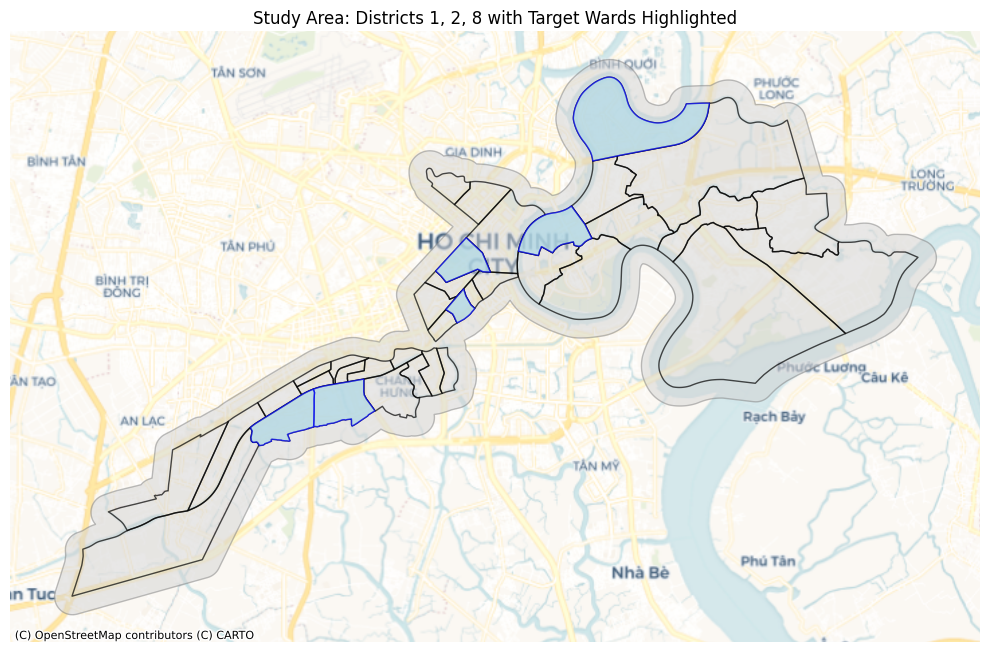
\includegraphics[keepaspectratio]{images/study_area.png}}

}

\caption{Study Area}

\end{figure}%

\begin{figure}[H]

{\centering \pandocbounded{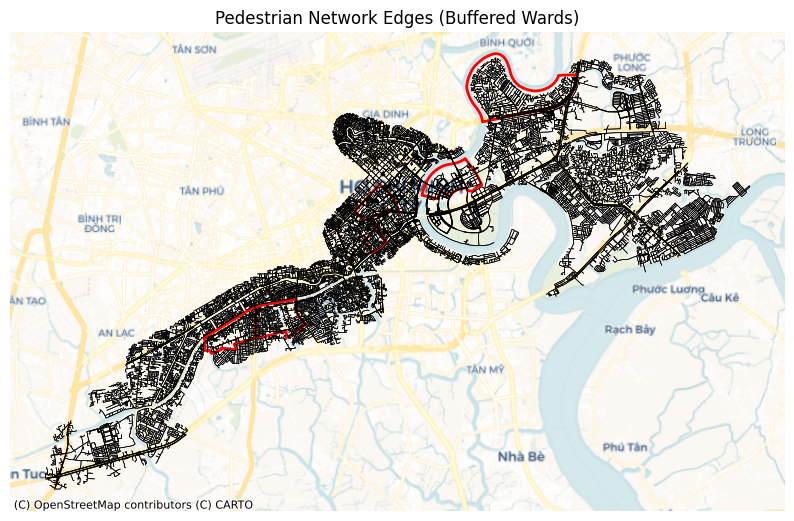
\includegraphics[keepaspectratio]{images/network_area.png}}

}

\caption{Network Area}

\end{figure}%

\section{Street-Level Imagery}\label{street-level-imagery}

GSV samples generated 23,806 points from 500-meter buffered wards of
interest at 50-meter intervals. Metadata contained 20,457 images, an
unfortunate 14.07\% decrease due to interruptions, but nonetheless
providing sufficient density for training streetscape indeces and
validating segmentation outputs within wards of interest.

\section{Remote Sensing Rasters}\label{remote-sensing-rasters}

The satellite data was extracted from several different sources:

\textbf{Landsat 8 / 9 (30m resolution, dry months December thru April,
2023--2025)}

\begin{itemize}
\item
  LST ST\_B10 Band
\item
  Emissivity ST\_EMIS Band
\item
  Red SR\_B4 Band
\item
  Near Infrared (NIR) SR\_B5 Band
\item
  QA\_PIXEL Band
\end{itemize}

\textbf{JAXA LULC (10m resolution, 2025)}

\begin{itemize}
\tightlist
\item
  Land Cover
\end{itemize}

\textbf{JAXA PALSAR-2 (ScanSAR, 50m resolution, 2025)}

\begin{itemize}
\item
  HH Polarization
\item
  HV Polarization
\item
  Observation Date / Time
\item
  Local Incidence Angle
\item
  Mask / Flag
\end{itemize}

\textbf{ALSO World 2D DSM (30m resolution, 2025)}

\begin{itemize}
\item
  Elevation
\item
  Mask
\item
  Stacking Number
\end{itemize}

\chapter{III. Methodologies}\label{iii.-methodologies}

In the interest of computational efficiency, all notebooks and scripting
were offloaded from local into cloud computing using Google's Colab.
Combining only Landsat rasters into a composite was completed in ArcGIS
v3.4.

\section{Image Segmentation and Superclass
Mapping}\label{image-segmentation-and-superclass-mapping}

GSV images were processed using a model trained on Southeast Asian
cities, Mask2Former Mapillary Vistas
(\texttt{facebook/mask2former-swin-large-mapillary-vistas-semantic}),
accessed via Hugging Face with an API token. It contains 66 object
categories for semantic segmentation primed for street-level scene
analysis for complex urban cities like Sài Gòn.

GSV images were 640 x 640 pixel resolution, ideally, panoramic images
would have been preferable, but due to cost restraints, the static
imagery was made to dynamically alter the header to be front-facing.

To improve interpretability and stability for index construction, raw
segmentation classes were remapped into seven superclasses:

\begin{longtable}[]{@{}ll@{}}
\caption{Superclass Mappings}\tabularnewline
\toprule\noalign{}
Mapping & Superclass \\
\midrule\noalign{}
\endfirsthead
\toprule\noalign{}
Mapping & Superclass \\
\midrule\noalign{}
\endhead
\bottomrule\noalign{}
\endlastfoot
0 & Other \\
1 & Vegetation \\
2 & Sky \\
3 & Building \\
4 & Pavement / Road \\
5 & Water \\
6 & Vehicle / Street Clutter \\
\end{longtable}

\begin{figure}[H]

{\centering \pandocbounded{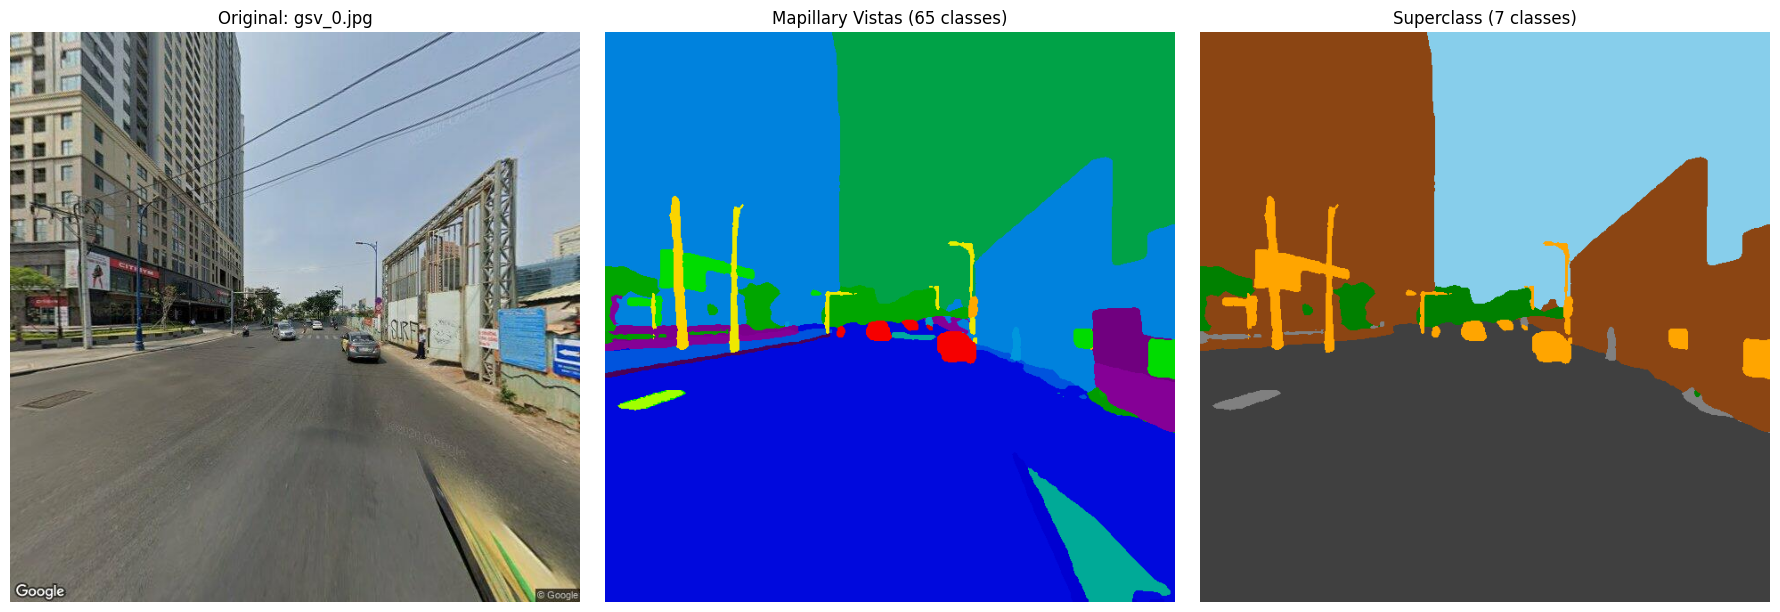
\includegraphics[keepaspectratio]{images/segmentation.png}}

}

\caption{Segmentation Process}

\end{figure}%

\section{Engineering Indeces}\label{engineering-indeces}

The final merged superclass imagery was used to create predictive
features:

\textbf{Green View Index (GVI):} Proportion of vegetation.

\textbf{Sky View Index (SVI):} Proportion of sky.

\textbf{Building View Index (BVI):} Proportion of building.

\textbf{Hardscape Index:} Combining building, pavement / road, and
vehicle / clutter classes.

\begin{figure}[H]

{\centering \pandocbounded{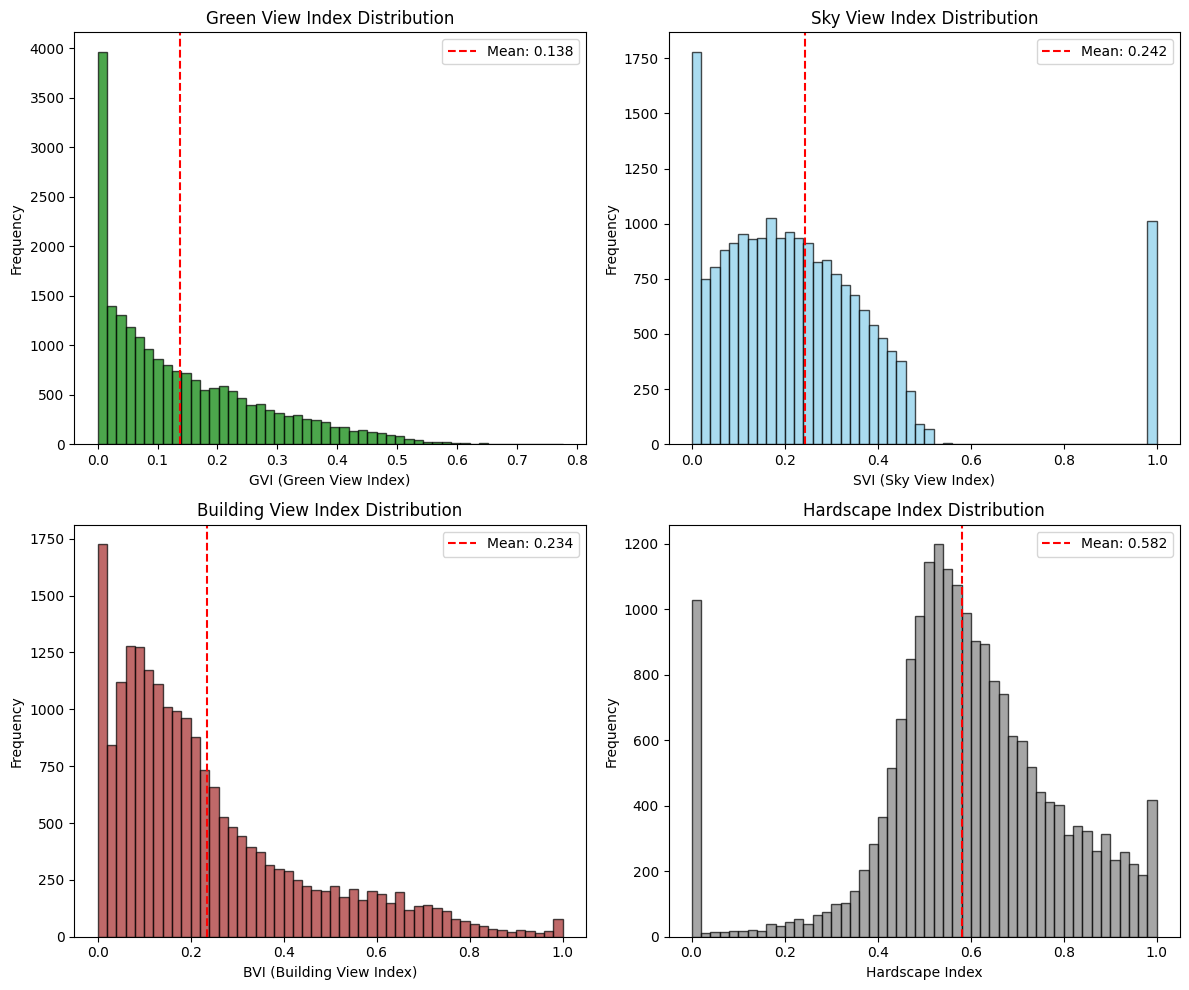
\includegraphics[keepaspectratio]{images/gsv_results.png}}

}

\caption{GSV-Derived Features}

\end{figure}%

\section{Raster Extraction}\label{raster-extraction}

The collection of Landsat rasters moved through the below workflow in
this order:

\begin{enumerate}
\def\labelenumi{\arabic{enumi}.}
\tightlist
\item
  Create Mosaic Dataset (Data Management)
\item
  Make Mosaic Layer (Data Management)
\item
  Cell Statistics (Spatial Analyst)
\item
  Raster Calculator (Spatial Analyst)
\item
  Copy Raster (Data Management)
\item
  Composite Bands (Data Management)
\end{enumerate}

A mosaic dataset was created to combine and stitch together 64 scenes
from 2023 thru 2025 during dry season months December thru April.

The different mosaic layers were isolated, with maximum LST and averages
for other layers. This was to process individual cell statistics to
convert DN raw values and re-scale, and raster calculations to calculate
NDVI and alter LST from Kelvin to Celsius. Only the QA\_PIXEL band was
acquired through the 5th tool.

Two extraction products were used for the rasters, one for the GSV
sample points and second for the entire network nodes. All raster values
were extracted for all nodes except for LST, where 0.0037\% of nodes
were unaccounted for, decreasing from 28,437 to 28,332 nodes.

\section{Model Design and Training}\label{model-design-and-training}

Two XGBoost models were trained using the \texttt{xgboost} Python
library, one as the full model including the rasters as well as the GSV
features for maximum predictive power, and second as the shared model
for real-world deployment using only the raster features.

\begin{Shaded}
\begin{Highlighting}[]
\CommentTok{\# Landsat features: thermal and vegetation indices.}
\NormalTok{LANDSAT\_FEATURES }\OperatorTok{=}\NormalTok{ [}
    \StringTok{"ndvi"}\NormalTok{,}
    \StringTok{"emissivity"}
\NormalTok{]}

\CommentTok{\# PALSAR features: radar backscatter and texture.}
\NormalTok{PALSAR\_FEATURES }\OperatorTok{=}\NormalTok{ [}
    \StringTok{"palsar\_hh\_db"}\NormalTok{,}
    \StringTok{"palsar\_hv\_db"}\NormalTok{,}
    \StringTok{"palsar\_hv\_hh\_ratio"}\NormalTok{,}
    \StringTok{"palsar\_glcm\_contrast"}\NormalTok{,}
    \StringTok{"palsar\_glcm\_homogeneity"}\NormalTok{,}
    \StringTok{"palsar\_glcm\_energy"}
\NormalTok{]}

\CommentTok{\# DSM features: elevation and sky view.}
\NormalTok{DSM\_FEATURES }\OperatorTok{=}\NormalTok{ [}
    \StringTok{"elevation\_m"}\NormalTok{,}
    \StringTok{"sky\_view\_factor"}
\NormalTok{]}

\CommentTok{\# Landcover features.}
\NormalTok{LANDCOVER\_FEATURES }\OperatorTok{=}\NormalTok{ [}
    \StringTok{"landcover\_class"}
\NormalTok{]}

\CommentTok{\# GSV segmentation features: visual indices from street imagery.}
\NormalTok{GSV\_SEGMENTATION\_FEATURES }\OperatorTok{=}\NormalTok{ [}
    \StringTok{"pct\_vegetation"}\NormalTok{,}
    \StringTok{"pct\_water"}\NormalTok{,}
\NormalTok{]}

\CommentTok{\# GSV derived features: computed indices.}
\NormalTok{GSV\_DERIVED\_FEATURES }\OperatorTok{=}\NormalTok{ [}
    \StringTok{"gvi"}\NormalTok{,}
    \StringTok{"svi"}\NormalTok{,}
    \StringTok{"bvi"}\NormalTok{,}
    \StringTok{"hardscape\_index"}
\NormalTok{]}

\CommentTok{\# Location features: administrative boundaries.}
\NormalTok{LOCATION\_FEATURES }\OperatorTok{=}\NormalTok{ [}
    \StringTok{"district"}\NormalTok{,}
    \StringTok{"ward"}
\NormalTok{]}
\end{Highlighting}
\end{Shaded}

The XGBoost parameters were carefully selected and to balance
complexity, learning speed, and regularization to prevent overfitting
while still capturing the complex, non-linear mechanisms that impact
LST, and are as follows:

\texttt{random.seed(42)}

\texttt{n\_estimators}: 500

\texttt{max\_depth}: 6

\texttt{learning\_rate}: 0.05

\texttt{subsample}: 0.8

\texttt{colsample\_bytree}: 0.8

\texttt{min\_child\_weight}: 3

\texttt{reg\_alpha}: 0.1

\texttt{reg\_lambda}: 1.0

\texttt{random\_state}: 42

\texttt{n\_jobs}: -1

\texttt{early\_stopping\_rounds}: 50

\section{Node Prediction and Routing}\label{node-prediction-and-routing}

A patchwork approach was pursued, using the GSV model to predict within
wards of interest and the shared raster-only model to predict outside of
those wards.

After generating predictions for network nodes a prediction raster was
derived from them and interpolated to create a hybrid cost surface. The
raster resolution was 0.0001 degrees and 2,266 x 1,409 pixel resolution
clipped to the area of interest encompassing the districts and a
Gaussian blur was applied to smooth out streak artifacts.

Dijkstra's algorithm was implemented, assigning heat edge costs by
combining normalized length and temperature to support three route types
with tunable heat penalty and reward parameters: shortest, coolest with
a temperature penalty, and hottest with an inverted temperature penalty
to reward.

\begin{Shaded}
\begin{Highlighting}[]
\CommentTok{\# Heat weights.}
\ControlFlowTok{for}\NormalTok{ u, v, data }\KeywordTok{in}\NormalTok{ G\_undirected.edges(data }\OperatorTok{=} \VariableTok{True}\NormalTok{):}
\NormalTok{    avg\_lst }\OperatorTok{=}\NormalTok{ data[}\StringTok{"avg\_lst"}\NormalTok{]}
\NormalTok{    length  }\OperatorTok{=}\NormalTok{ data[}\StringTok{"length"}\NormalTok{]}

    \CommentTok{\# Normalize temperature to [0, 1].}
\NormalTok{    temp\_norm }\OperatorTok{=}\NormalTok{ (avg\_lst }\OperatorTok{{-}}\NormalTok{ lst\_min) }\OperatorTok{/}\NormalTok{ lst\_range}

    \CommentTok{\# Normalize length relative to mean edge length.}
\NormalTok{    length\_norm }\OperatorTok{=}\NormalTok{ length }\OperatorTok{/}\NormalTok{ len\_mean}

    \CommentTok{\# Tune lambda.}
\NormalTok{    lambda\_cool }\OperatorTok{=} \FloatTok{10.0} \CommentTok{\# How much to penalize heat.}
\NormalTok{    lambda\_hot  }\OperatorTok{=} \FloatTok{10.0} \CommentTok{\# How much to reward heat.}

    \CommentTok{\# Cool Cost: shorter + cooler (high temperature = high penalty).}
\NormalTok{    data[}\StringTok{"cool\_cost"}\NormalTok{] }\OperatorTok{=}\NormalTok{ length\_norm }\OperatorTok{+}\NormalTok{ lambda\_cool }\OperatorTok{*}\NormalTok{ temp\_norm}

    \CommentTok{\# Hot Cost: shorter + hotter (invert temp\_norm).}
\NormalTok{    data[}\StringTok{"hot\_cost"}\NormalTok{] }\OperatorTok{=}\NormalTok{ length\_norm }\OperatorTok{+}\NormalTok{ lambda\_hot }\OperatorTok{*}\NormalTok{ (}\FloatTok{1.0} \OperatorTok{{-}}\NormalTok{ temp\_norm)}
\end{Highlighting}
\end{Shaded}

\begin{Shaded}
\begin{Highlighting}[]
\CommentTok{\# Routing helpers.}
\KeywordTok{def}\NormalTok{ get\_hottest\_route(G, start, end):}
    \CommentTok{"""Shortest{-}ish but biased toward hottest edges."""}
    \ControlFlowTok{try}\NormalTok{:}
\NormalTok{        path }\OperatorTok{=}\NormalTok{ nx.dijkstra\_path(G, start, end, weight }\OperatorTok{=} \StringTok{"hot\_cost"}\NormalTok{)}
\NormalTok{        cost }\OperatorTok{=}\NormalTok{ nx.dijkstra\_path\_length(G, start, end, weight }\OperatorTok{=} \StringTok{"hot\_cost"}\NormalTok{)}
\NormalTok{        dist }\OperatorTok{=}\NormalTok{ nx.path\_weight(G, path, weight }\OperatorTok{=} \StringTok{"length"}\NormalTok{)}
        \ControlFlowTok{return}\NormalTok{ path, cost, dist}
    \ControlFlowTok{except}\NormalTok{ nx.NetworkXNoPath:}
        \ControlFlowTok{return} \VariableTok{None}\NormalTok{, }\VariableTok{None}\NormalTok{, }\VariableTok{None}

\KeywordTok{def}\NormalTok{ get\_coolest\_route(G, start, end):}
    \CommentTok{"""Shortest{-}ish but biased toward coolest edges."""}
    \ControlFlowTok{try}\NormalTok{:}
\NormalTok{        path }\OperatorTok{=}\NormalTok{ nx.dijkstra\_path(G, start, end, weight }\OperatorTok{=} \StringTok{"cool\_cost"}\NormalTok{)}
\NormalTok{        cost }\OperatorTok{=}\NormalTok{ nx.dijkstra\_path\_length(G, start, end, weight }\OperatorTok{=} \StringTok{"cool\_cost"}\NormalTok{)}
\NormalTok{        dist }\OperatorTok{=}\NormalTok{ nx.path\_weight(G, path, weight }\OperatorTok{=} \StringTok{"length"}\NormalTok{)}
        \ControlFlowTok{return}\NormalTok{ path, cost, dist}
    \ControlFlowTok{except}\NormalTok{ nx.NetworkXNoPath:}
        \ControlFlowTok{return} \VariableTok{None}\NormalTok{, }\VariableTok{None}\NormalTok{, }\VariableTok{None}

\KeywordTok{def}\NormalTok{ get\_shortest\_route(G, start, end):}
    \CommentTok{"""}
\CommentTok{    Returns shortest walking path.}
\CommentTok{    """}
    \ControlFlowTok{try}\NormalTok{:}
\NormalTok{        path }\OperatorTok{=}\NormalTok{ nx.shortest\_path(G, start, end, weight }\OperatorTok{=} \StringTok{"length"}\NormalTok{)}
\NormalTok{        dist }\OperatorTok{=}\NormalTok{ nx.path\_weight(G, path, weight }\OperatorTok{=} \StringTok{"length"}\NormalTok{)}
        \ControlFlowTok{return}\NormalTok{ path, dist}
    \ControlFlowTok{except}\NormalTok{ nx.NetworkXNoPath:}
        \ControlFlowTok{return} \VariableTok{None}\NormalTok{, }\VariableTok{None}
\end{Highlighting}
\end{Shaded}

\chapter{IV. Results}\label{iv.-results}

\section{Model Performance}\label{model-performance}

\begin{longtable}[]{@{}lll@{}}
\caption{Full Model Cross-Validation Results}\tabularnewline
\toprule\noalign{}
Statistic & Value & Error \\
\midrule\noalign{}
\endfirsthead
\toprule\noalign{}
Statistic & Value & Error \\
\midrule\noalign{}
\endhead
\bottomrule\noalign{}
\endlastfoot
RMSE & 0.7001 & 0.0115 \\
R² & 0.7959 & 0.0089 \\
MAE & 0.5106 & 0.0103 \\
\end{longtable}

\begin{longtable}[]{@{}lll@{}}
\caption{Shared Model Cross-Validation Results}\tabularnewline
\toprule\noalign{}
Statistic & Value & Error \\
\midrule\noalign{}
\endfirsthead
\toprule\noalign{}
Statistic & Value & Error \\
\midrule\noalign{}
\endhead
\bottomrule\noalign{}
\endlastfoot
RMSE & 0.7117 & 0.0173 \\
R² & 0.7892 & 0.0083 \\
MAE & 0.5105 & 0.0141 \\
\end{longtable}

The difference between the two models is marginal, with a 0.0116 change
in RMSE, 0.0067 change in R², and 0.0001 change in MAE. The shared model
has a slight degradation compared to the full model, suggesting that GSV
provides micro-scale refinement.

\section{Feature Importance}\label{feature-importance}

\begin{longtable}[]{@{}ll@{}}
\caption{Full Model Feature Importance}\tabularnewline
\toprule\noalign{}
\textbf{Feature} & \textbf{Importance} \\
\midrule\noalign{}
\endfirsthead
\toprule\noalign{}
\textbf{Feature} & \textbf{Importance} \\
\midrule\noalign{}
\endhead
\bottomrule\noalign{}
\endlastfoot
emissivity & 0.2314 \\
ndvi & 0.2167 \\
landcover\_class & 0.1979 \\
elevation\_m & 0.0486 \\
pct\_vegetation & 0.0416 \\
svi & 0.0359 \\
sky\_view\_factor & 0.0270 \\
pct\_water & 0.0256 \\
palsar\_hh\_db & 0.0244 \\
gvi & 0.0244 \\
\end{longtable}

\begin{longtable}[]{@{}ll@{}}
\caption{Shared Model Feature Importance}\tabularnewline
\toprule\noalign{}
\textbf{Feature} & \textbf{Importance} \\
\midrule\noalign{}
\endfirsthead
\toprule\noalign{}
\textbf{Feature} & \textbf{Importance} \\
\midrule\noalign{}
\endhead
\bottomrule\noalign{}
\endlastfoot
emissivity & 0.2314 \\
landcover\_class & 0.2167 \\
ndvi & 0.1979 \\
elevation\_m & 0.0486 \\
sky\_view\_factor & 0.0416 \\
palsar\_hv\_db & 0.0359 \\
palsar\_hh\_db & 0.0270 \\
palsar\_glcm\_contrast & 0.0256 \\
palsar\_hv\_hh\_ratio & 0.0244 \\
palsar\_glcm\_homogeneity & 0.0244 \\
\end{longtable}

The dominant predictors were consistent across both models. Emissivity,
NDVI, and land cover class ranked highest, followed by elevation and
SAR-derived structure (HH/HV backscatter and GLCM texture). In the full
model, streetscape variables (e.g.~vegetation and sky-related measures)
contributed additional explanatory signal.

\section{Node Prediction Coverage}\label{node-prediction-coverage}

\begin{longtable}[]{@{}llll@{}}
\caption{LST Prediction Statistics}\tabularnewline
\toprule\noalign{}
Minimum & Mean & Maximum & Standard Deviation \\
\midrule\noalign{}
\endfirsthead
\toprule\noalign{}
Minimum & Mean & Maximum & Standard Deviation \\
\midrule\noalign{}
\endhead
\bottomrule\noalign{}
\endlastfoot
35.44°C & 40.84°C & 46.28°C & 1.76°C \\
\end{longtable}

\begin{figure}[H]

{\centering \pandocbounded{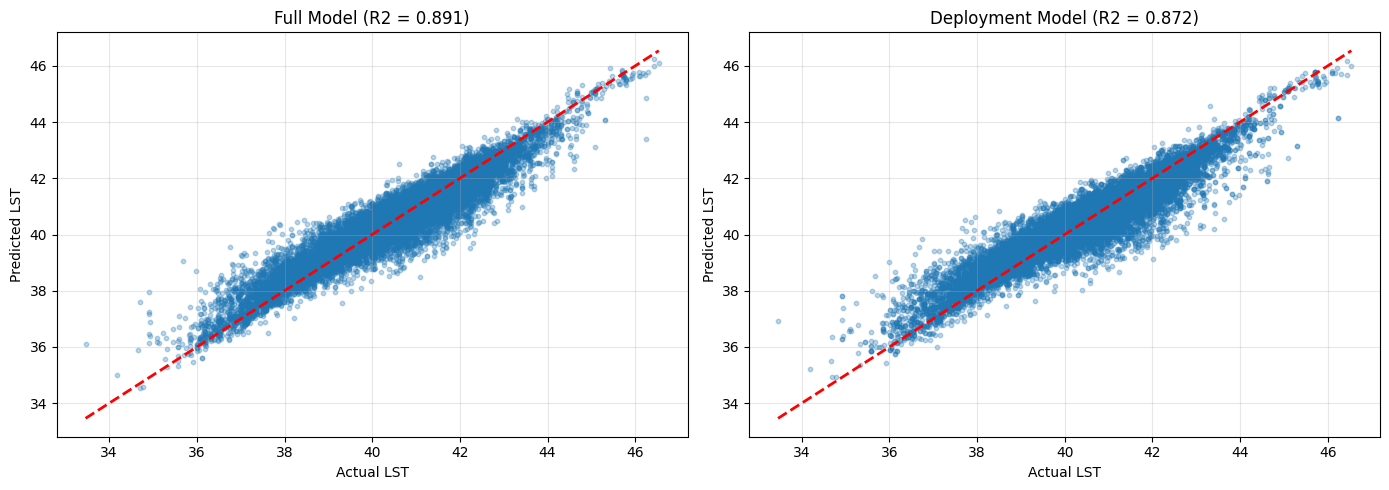
\includegraphics[keepaspectratio]{images/LST_predictions.png}}

}

\caption{LST Predictions Scatter Plot}

\end{figure}%

\begin{figure}[H]

{\centering \pandocbounded{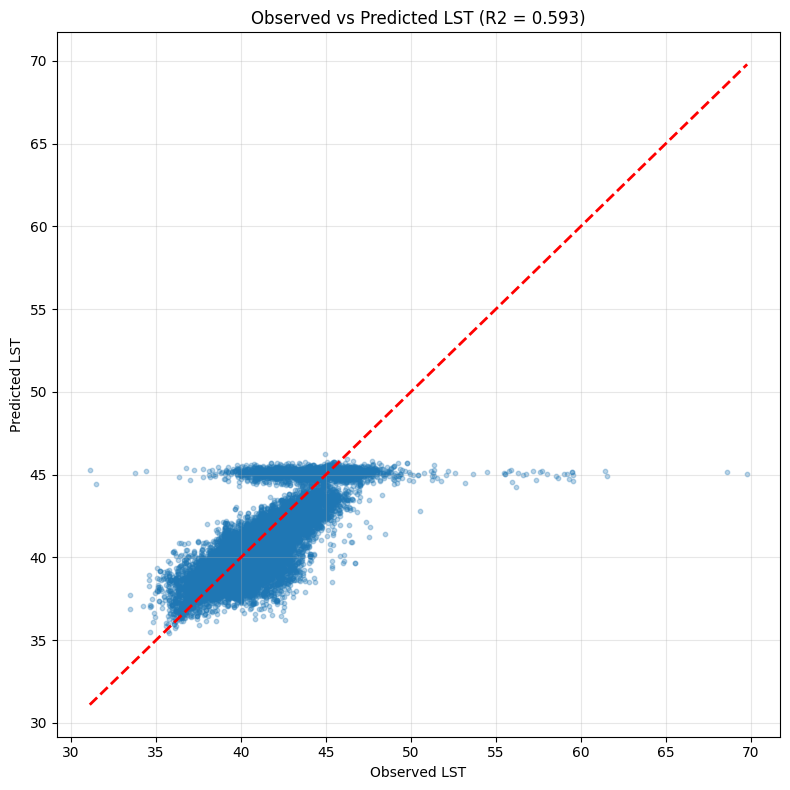
\includegraphics[keepaspectratio]{images/LST_observed_predicted.png}}

}

\caption{LST Observed vs.~Predicted Scatter Plot}

\end{figure}%

\begin{figure}[H]

{\centering \pandocbounded{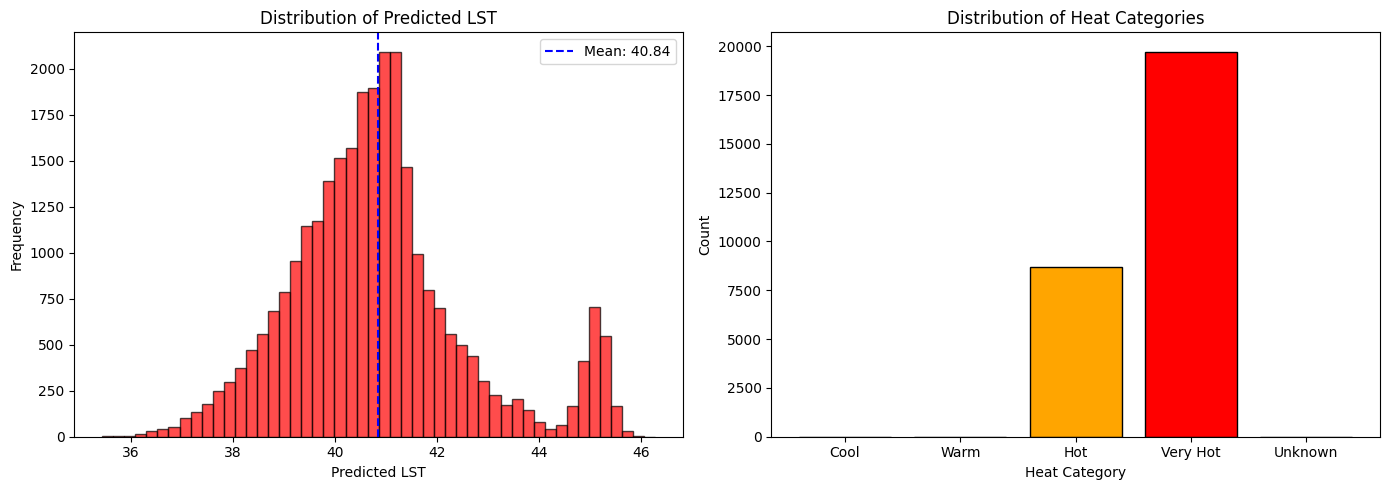
\includegraphics[keepaspectratio]{images/LST_distribution.png}}

}

\caption{LST Predicted Map}

\end{figure}%

\begin{figure}[H]

{\centering \pandocbounded{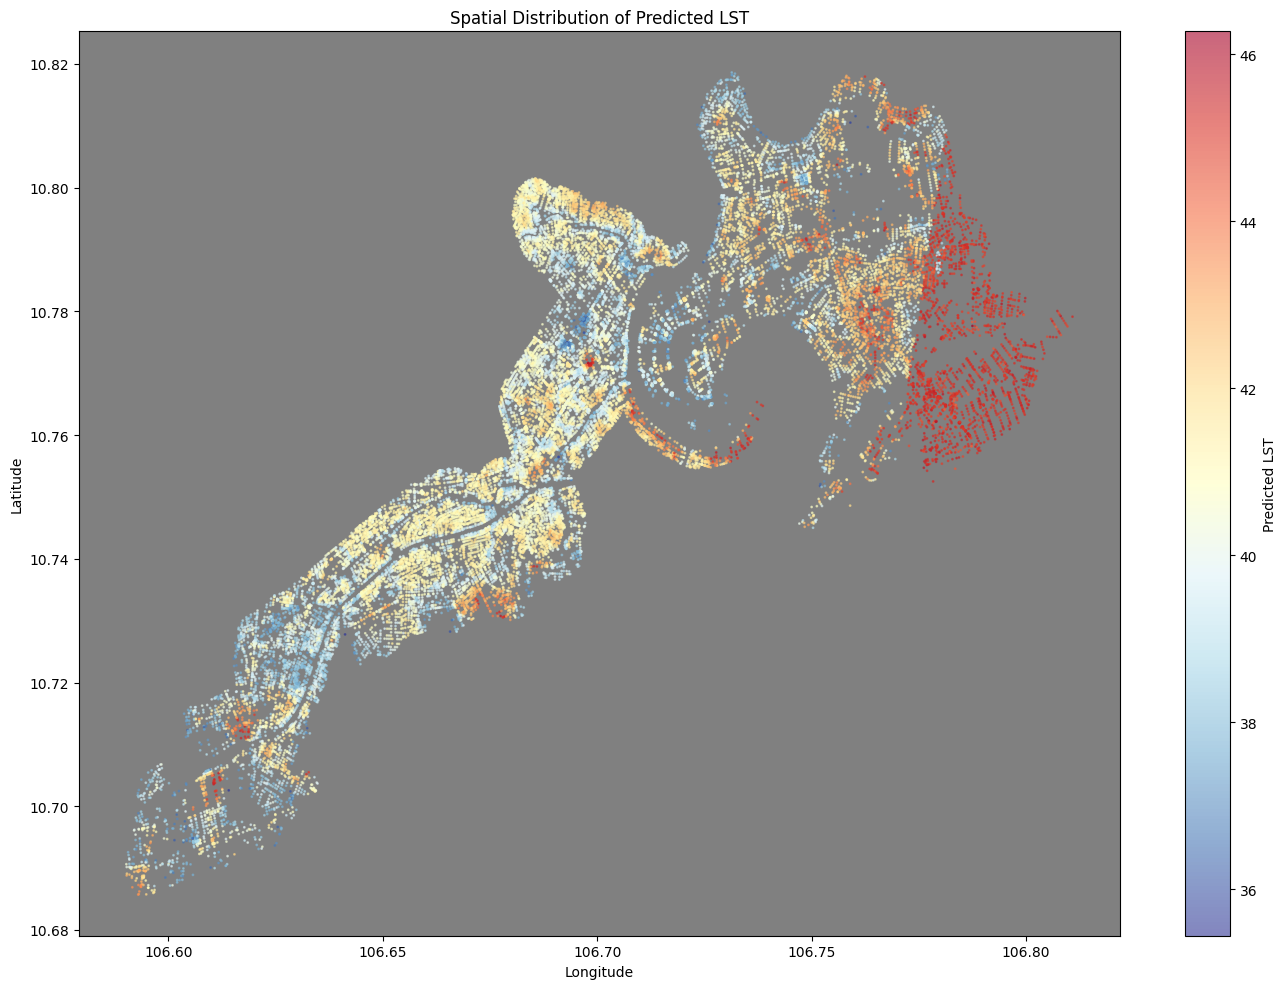
\includegraphics[keepaspectratio]{images/LST_predicted_map.png}}

}

\caption{LST Predicted Map}

\end{figure}%

When compared against nodes with extracted Landsat LST, performance was
lower (RMSE 1.3127, R² 0.5929, MAE 0.8487), likely reflecting scale
mismatch between point-linked training data and node-level evaluation
plus spatial and sensor aggregation effects.

\section{Routing Outcomes}\label{routing-outcomes}

The coolest route increases travel distance but reduces both mean and
peak exposure, demonstrating tangible potential for heat-resilient
mobility guidance.

\begin{figure}[H]

{\centering \pandocbounded{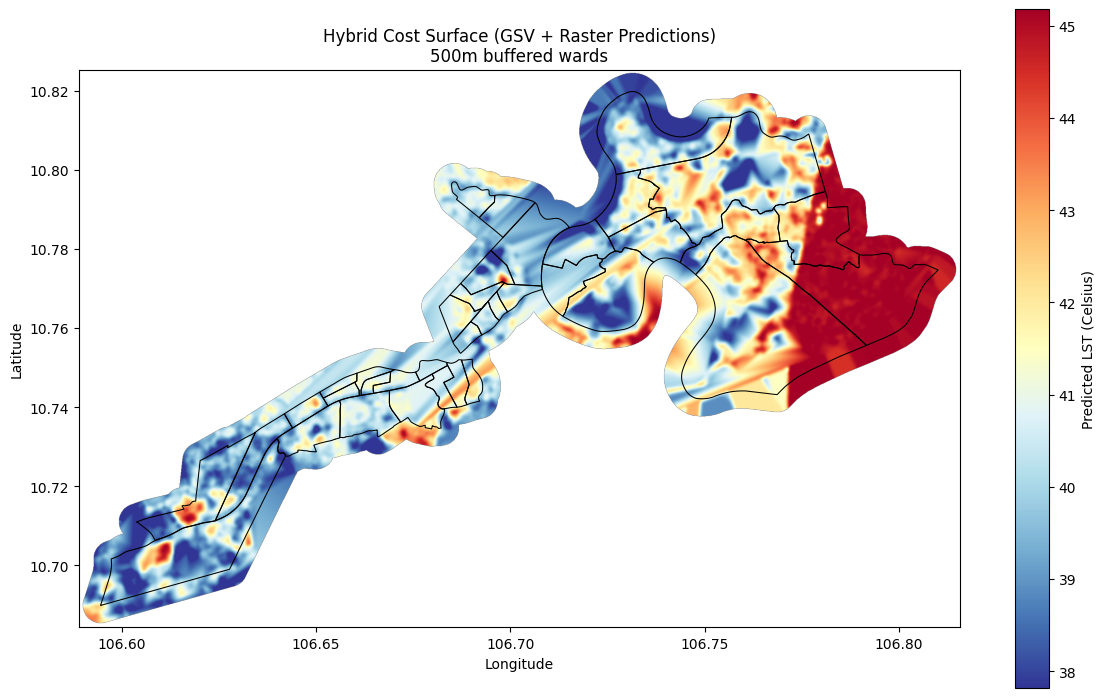
\includegraphics[keepaspectratio]{images/hybrid_raster.png}}

}

\caption{Hybrid Cost Surface Raster}

\end{figure}%

\begin{figure}[H]

{\centering \pandocbounded{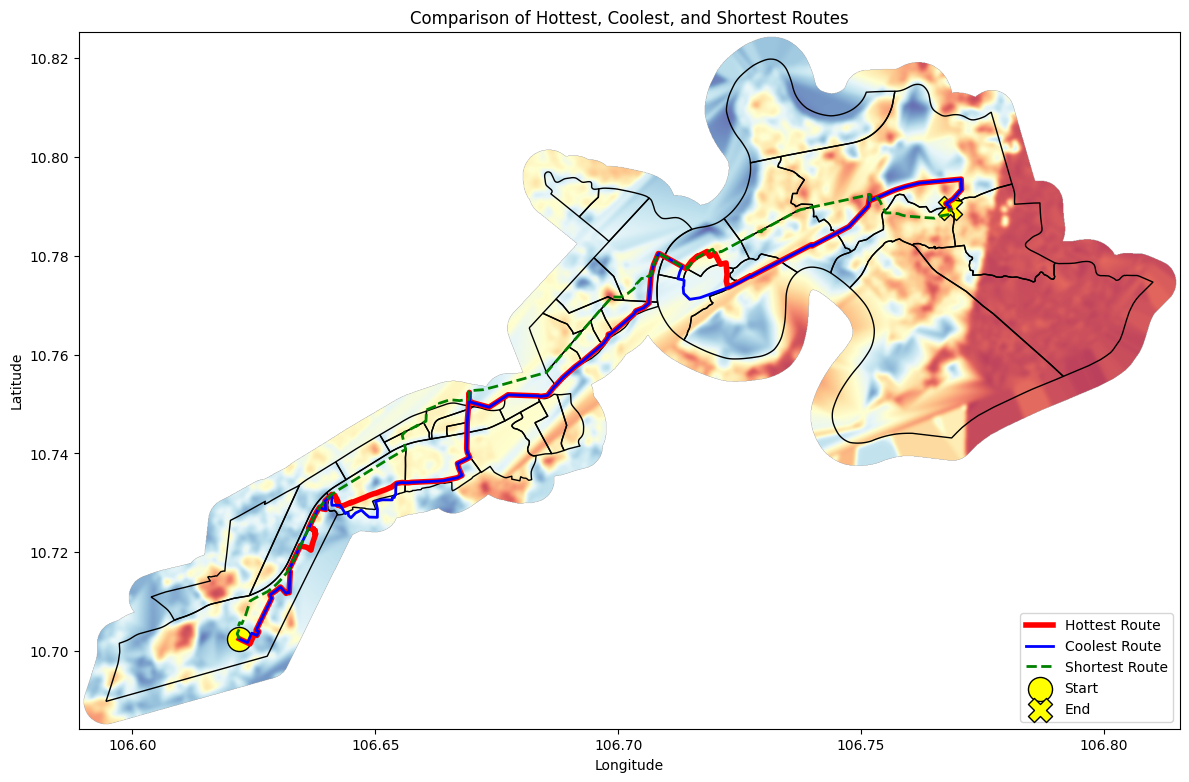
\includegraphics[keepaspectratio]{images/routes.png}}

}

\caption{Dijkstra Routes: Hottest, Coolest, and Shortest}

\end{figure}%

\begin{figure}[H]

{\centering \pandocbounded{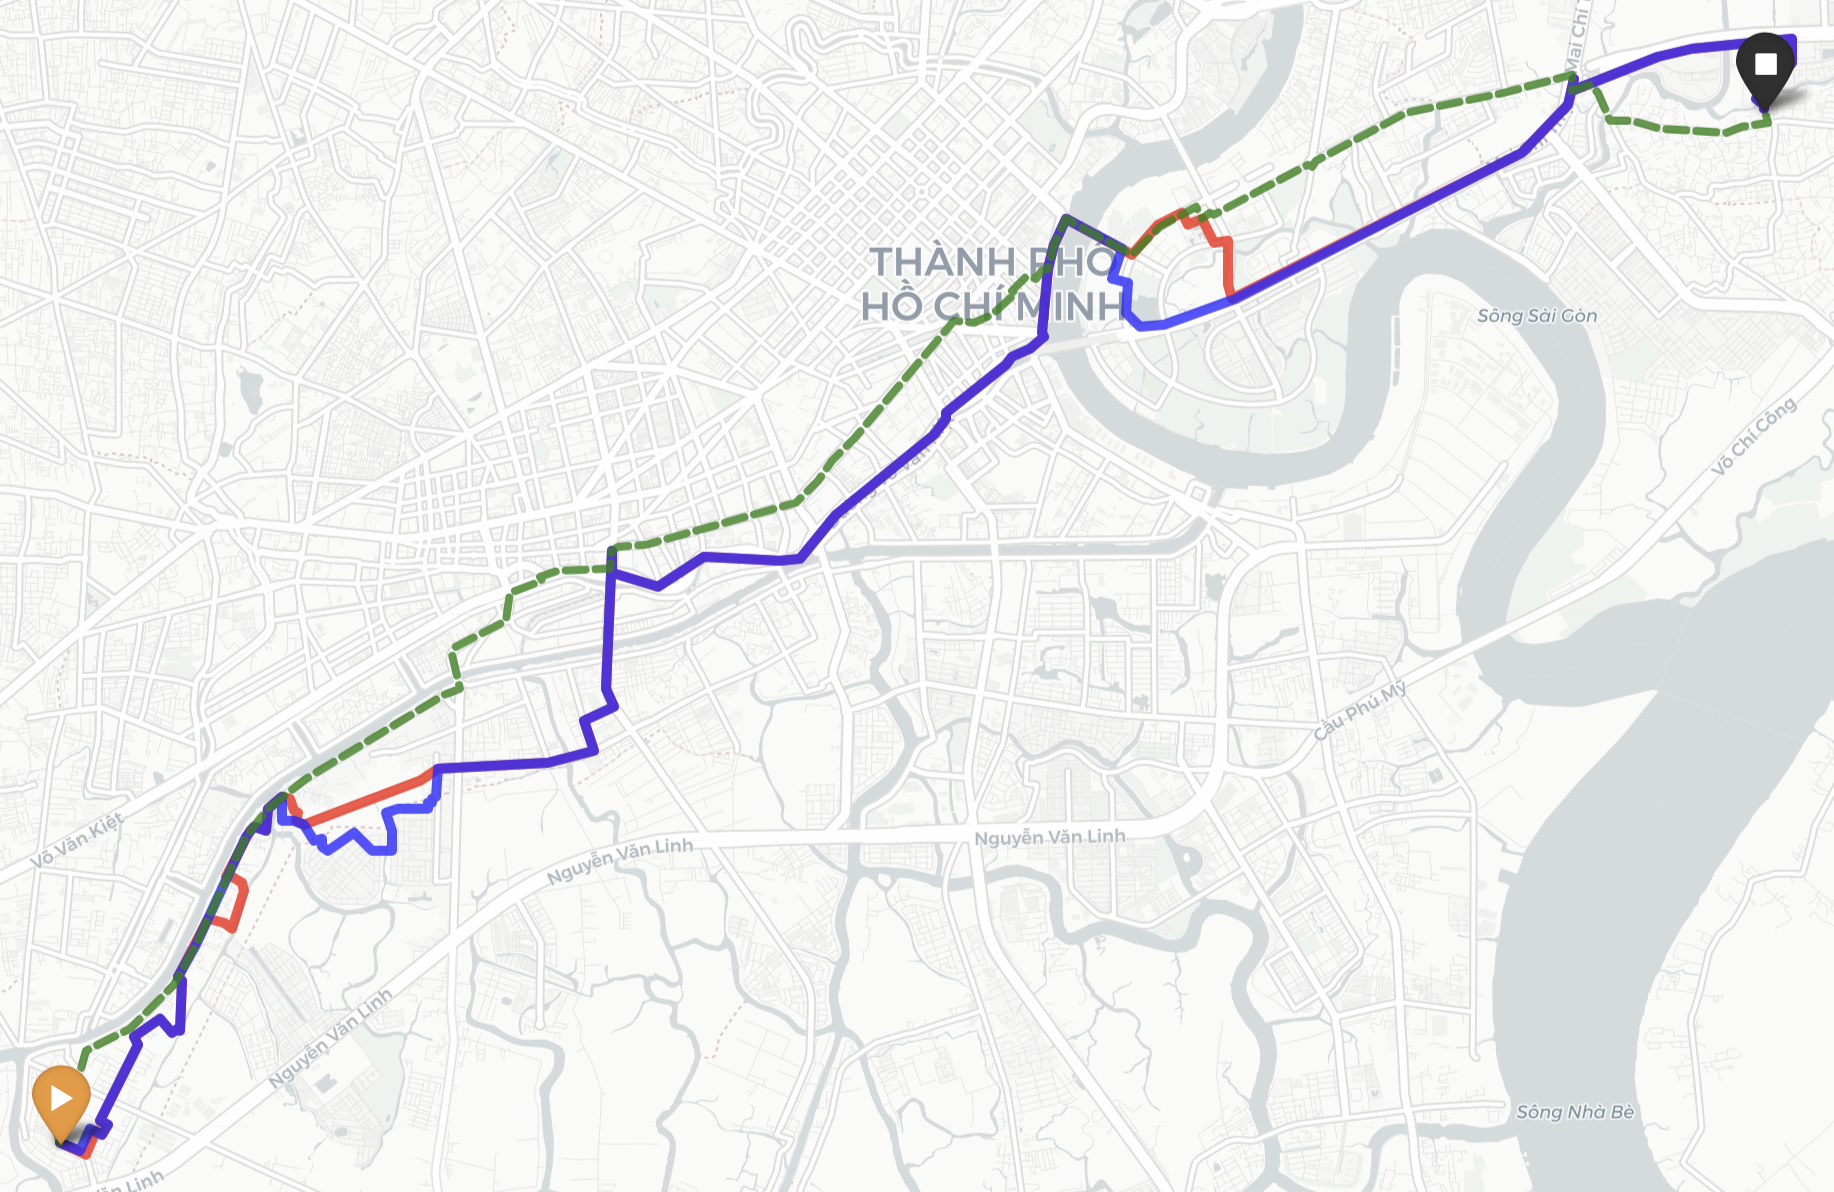
\includegraphics[keepaspectratio]{images/carto_map.png}}

}

\caption{Route Map}

\end{figure}%

\begin{longtable}[]{@{}llll@{}}
\caption{Routing Results}\tabularnewline
\toprule\noalign{}
Route & Distance (km) & Average LST & Maximum LST \\
\midrule\noalign{}
\endfirsthead
\toprule\noalign{}
Route & Distance (km) & Average LST & Maximum LST \\
\midrule\noalign{}
\endhead
\bottomrule\noalign{}
\endlastfoot
Shortest & 22.00 & 40.63°C & 45.41°C \\
Coolest & 27.83 & 40.20°C & 43.95°C \\
Hottest & 27.38 & 40.40°C & 43.95°C \\
\end{longtable}

\chapter{V. Discussion and
Limitations}\label{v.-discussion-and-limitations}

Hot Hẻm demonstrates a scalable approach for integrating human-scale
streetscape morphology with city-scale remote sensing to operationalize
pedestrian heat risk. The small performance gap between full and
deployment models suggests that the system remains robust even in areas
with sparse GSV coverage.

Two limitations merit emphasis. First, temporal alignment between GSV
acquisition and satellite composites may introduce noise in model
relationships. Second, the current heat-category thresholds appear to
skew heavily toward ``Hot/Very Hot,'' suggesting that categorical
calibration (e.g., quantile-based or health-relevant thresholds) should
be refined prior to policy-facing deployment.

\chapter{VI. Conclusion}\label{vi.-conclusion}

This project delivers a reproducible, multi-scale GeoAI pipeline for
heat-weighted pedestrian routing in Ho Chi Minh City. By combining
GSV-derived segmentation indices with Landsat thermal variables, JAXA
SAR structure, and DSM terrain context, the framework achieves strong
predictive accuracy and enables practical routing alternatives that
reduce heat exposure. Future extensions should include threshold
calibration, multi-season modeling, and uncertainty-aware routing to
further strengthen real-world applicability.




\end{document}
